\documentclass[10pt,a4paper]{article}
\usepackage[margin=2.1cm]{geometry}
\usepackage{amsmath,amssymb}
\usepackage{booktabs}
\usepackage{graphicx}
\usepackage{caption}
\usepackage[hidelinks]{hyperref}
\usepackage{microtype}
\usepackage{titlesec}
\titlespacing*{\section}{0pt}{9pt}{4pt}
\titleformat{\section}{\normalfont\large\bfseries}{\thesection}{0.8em}{}
\captionsetup{font=small,labelfont=bf,skip=4pt}
\setlength{\parskip}{2pt}

\title{\vspace{-1.6cm}\large\textbf{Zero-slack-qubit improvements to the QUBO formulation of\\
Borowski et al.\ (ICCS 2020) for the Vehicle Routing Problem with Time Windows}}
\author{\normalsize Mahmoud Naderi \,---\, July 14, 2026}
\date{}

\begin{document}
\maketitle
\vspace{-1.4cm}

\section{Baseline: the FQS formulation}

The paper's Full QUBO Solver (FQS) encodes CVRPTW monolithically with binaries
$x_{v,j,k}=1$ iff vehicle $v$ serves customer $j$ as its $k$-th stop
($k=1,\dots,N$), i.e.\ $O(MN^2)$ variables for $M$ vehicles and $N$ customers:
\begin{equation}
\begin{split}
H_{\mathrm{FQS}} \;=\;
\sum_{v}\Bigl[\sum_{j} \bigl(d_{0j}\,x_{v,j,1} + d_{j0}\,x_{v,j,N}\bigr)
+ \sum_{k=1}^{N-1}\sum_{i\neq j} d_{ij}\,x_{v,i,k}\,x_{v,j,k+1}\Bigr]\\[-2pt]
+\, A\sum_{j}\Bigl(\sum_{v,k} x_{v,j,k}-1\Bigr)^{2}
+\, A\sum_{v,k}\sum_{i<j} x_{v,i,k}\,x_{v,j,k},
\end{split}
\label{eq:fqs}
\end{equation}
with $A = 2N d_{\max}$. Two structural problems: the variable count explodes
(a Solomon-100 instance needs $\sim$$10^5$ binaries), and neither time windows
nor capacity appear in the QUBO at all --- the paper handles them outside the
sampler, so FQS can return solutions that are structurally valid but
TW-infeasible. Everything below attacks these two problems \emph{without
spending any extra qubits} (no slack binaries anywhere).

\section{Improved formulation}

\paragraph{Decomposition.} Cluster-first, route-second: one assignment QUBO
over $y_{c,k}=1$ iff customer $c$ goes to vehicle $k$ ($NM$ variables), then
one independent open-TSP QUBO per resulting cluster ($n^2$ or $n(n-1)$
variables for a cluster of size $n$). The largest single BQM drops from
$O(MN^2)$ to $\max(NM,\,n_{\max}^2)$.

\paragraph{Assignment QUBO with unbalanced capacity penalization.}
\begin{equation}
H_{\mathrm{asg}} = \sum_{k}\sum_{c<c'}\bigl(D_{cc'} + W\,[\,\{c,c'\}\in\mathcal{M}\,]\bigr)\,y_{ck}y_{c'k}
+ \gamma\sum_{k,c} d_{0c}\,y_{ck}
+ A\sum_{c}\Bigl(\sum_{k}y_{ck}-1\Bigr)^{2}
+ \sum_{k}\bigl(-\lambda_1 h_k + \lambda_2 h_k^2\bigr),
\label{eq:asg}
\end{equation}
where $D_{cc'} = \tfrac12 d_{cc'} + \tfrac12\,|m_c-m_{c'}|\cdot d_{\max}/T$ is a
spatio-\emph{temporal} affinity ($m_c=(e_c+l_c)/2$ is the window midpoint, $T$
the horizon), and $h_k = C - \sum_c q_c\,y_{ck}$ is the residual capacity of
vehicle $k$. The usual way to encode $\sum_c q_c y_{ck}\le C$ needs
$\lceil\log_2 C\rceil$ slack binaries per vehicle; the unbalanced penalty
$-\lambda_1 h + \lambda_2 h^2$ is already quadratic in $y$, so it costs
\emph{zero} extra variables. It is asymmetric: mildly rewards spare capacity,
sharply punishes overload.

\paragraph{Time-window conflict pairs.} A directed pair $(i,j)$ can never be
consecutive if $e_i + s_i + \tau_{ij} > l_j$ (leave $i$ as early as possible,
still miss $j$'s deadline). This is precomputable classically, and enters both
stages at zero qubit cost: in each TSP QUBO every conflicting arc gets weight
$\tau_{ij} + \Gamma$ instead of $\tau_{ij}$; and (new in this round) pairs
conflicting in \emph{both} directions form the set $\mathcal{M}$ in
Eq.~\eqref{eq:asg}, penalized with weight $W$ when co-assigned. The
$\mathcal{M}$-penalty must be soft: two mutually conflicting customers can
still share a route with an intermediate stop between them.

\paragraph{Per-cluster open TSP, one-hot vs.\ domain-wall.} The one-hot
version over $x_{p,c}$ ($c$ visited at position $p$) is standard:
\begin{equation}
H_{\mathrm{tsp}} = \sum_{c}\bigl(\tau_{0c}\,x_{0,c} + \tau_{c0}\,x_{n-1,c}\bigr)
+ \sum_{p=0}^{n-2}\sum_{i\neq j}\tilde\tau_{ij}\,x_{p,i}\,x_{p+1,j}
+ A_2\sum_{p}\Bigl(\sum_c x_{p,c}-1\Bigr)^{2}
+ A_2\sum_{c}\Bigl(\sum_p x_{p,c}-1\Bigr)^{2},
\label{eq:tsp}
\end{equation}
with $\tilde\tau_{ij} = \tau_{ij} + \Gamma\,[\,(i,j)\ \text{conflict}\,]$. The
domain-wall encoding replaces each position's one-hot row by $n-1$ wall
variables $z_{p,k}$ via the affine map $x_{p,c} = \bar z_{p,c} - \bar
z_{p,c+1}$ (with $\bar z_{p,0}\equiv 1$, $\bar z_{p,n}\equiv 0$), i.e.\ $x = Bz
+ b_0$. Substituting into the \emph{unpenalized} objective $Q_x$ of
Eq.~\eqref{eq:tsp} gives
\begin{equation}
H_{\mathrm{dw}}(z) = z^\top\! B^\top\! Q_x B\, z + 2\,b_0^\top Q_x B\, z + b_0^\top Q_x b_0
\;+\; \kappa \sum_{p}\sum_{k} z_{p,k+1}\bigl(1 - z_{p,k}\bigr)
\;+\; A_c \sum_{c}\Bigl(\textstyle\sum_p x_{p,c}(z)-1\Bigr)^{2},
\label{eq:dw}
\end{equation}
which is $n(n-1)$ variables and, being an exact affine transform, has
\emph{identical energy to the one-hot QUBO on every valid tour}. I verified
this exhaustively: over all $5!$ tours of a random instance,
$\max|E_{\mathrm{onehot}} - E_{\mathrm{dw}}| = 5.6\times10^{-12}$, and both
equal the true tour length (\texttt{tests\_encoding.py}).

\paragraph{Exact-window coarsening (front end for $N=100$).} Merging customers
$i\!\to\!j$ into a super-node with $E = e_i$, $L = \min(l_i,\; l_j - s_i -
\tau_{ij})$, admissible iff $E\le L$, is both sound and complete (the paper-3
rule rejects sequenceable disjoint windows; the relaxed rule admits infeasible
merges). Duration $S = s_i + \tau_{ij} + s_j + \max(0,\, e_j - E - s_i -
\tau_{ij})$ upper-bounds the true duration for any start in $[E,L]$, so any
coarse-feasible route inflates to a feasible original route \emph{with no
repair step}. Super-nodes carry $(E,L,S,q)$ --- the same signature as a
customer --- so the QUBOs above run on the coarse instance unchanged.

\paragraph{Sample-pool utilization.} Annealers return distributions, not
argmins: the top-$K$ \emph{distinct} assignments from the sample pool are all
routed (with memoized cluster TSPs), keeping the best end-to-end feasible
solution. A coarse-level Clarke--Wright savings run sizes the fleet and
warm-starts the pool. Fleet sizes must come from TW-aware bounds ---
capacity-based bounds were proven infeasible on tight-window instances during
debugging.

\section{Validation}

I re-ran the entire bundled pipeline from scratch (Python 3.10, dimod 0.12,
\texttt{dwave-samplers} SA): the encoding equivalence test passes as claimed,
and all three experiments reproduce the bundled CSVs \emph{exactly} (bitwise-identical
metric columns; only wall times differ), as the SA sampler is seeded.
Two footnotes from the audit: the bundled README table reports RC101-$N$10
DECOMP-DW as 374.7 where its own CSV says 382.9, and it omits the RC101-$N$5
row --- both corrected in Table~\ref{tab:expA}. All results below are from my
re-run. \textbf{Caveat:} the sampler is D-Wave's \emph{classical} simulated
annealer (the standard control in this literature); no QPU access was
available. \texttt{run\_qpu.py} runs the same experiments unchanged on Leap
hardware.

\section{Results}

\paragraph{A --- head-to-head at annealer scale.} Truncated Solomon instances
at $N\in\{5,10\}$ (the sizes of the lineage's published quantum experiments),
identical budget for all methods (500 reads $\times$ 2000 sweeps),
TW-aware-greedy fleet sizing, exact optimum by brute force at $N=5$.

\begin{table}[h]\centering\small
\caption{Experiment A. \emph{vars} = total binaries; \emph{max BQM} = largest
single QUBO sampled; distances are the best TW/capacity-feasible decoded
solutions. Every method returned 100\% \emph{structurally} valid samples;
``infeasible'' means none of 500 valid samples respected the time windows.
DECOMP-OH rows are omitted: identical distances to DECOMP-DW with more
variables (e.g.\ 217 vs.\ 162 on C101-$N$10).}
\label{tab:expA}
\begin{tabular}{llrrrr}
\toprule
instance & method & vars & max BQM & best feas.\ dist & gap \\
\midrule
C101-$N$5 & exact opt. & --- & --- & 42.4 & --- \\
C101-$N$5 & FQS & 50 & 50 & 72.7 & 71.5\% \\
C101-$N$5 & DECOMP-DW & 50 & 10 & 74.7 & 76.2\% \\
\addlinespace[2pt]
C101-$N$10 & FQS & 300 & 300 & \textbf{infeasible} & n/a \\
C101-$N$10 & DECOMP-DW & 162 & 30 & 123.9 & n/a \\
\addlinespace[2pt]
R101-$N$5 & exact opt. & --- & --- & 156.3 & --- \\
R101-$N$5 & FQS & 75 & 75 & 156.4 & 0.1\% \\
R101-$N$5 & DECOMP-DW & 24 & 15 & 156.6 & 0.2\% \\
\addlinespace[2pt]
R101-$N$10 & FQS & 600 & 600 & \textbf{infeasible} & n/a \\
R101-$N$10 & DECOMP-DW & 99 & 60 & 312.1 & n/a \\
\addlinespace[2pt]
RC101-$N$5 & exact opt. & --- & --- & 89.1 & --- \\
RC101-$N$5 & FQS & 75 & 75 & 155.6 & 74.6\% \\
RC101-$N$5 & DECOMP-DW & 23 & 15 & 233.9 & 162.5\% \\
\addlinespace[2pt]
RC101-$N$10 & FQS & 500 & 500 & 410.3 & n/a \\
RC101-$N$10 & DECOMP-DW & 120 & 50 & 382.9 & n/a \\
\bottomrule
\end{tabular}
\end{table}

At $N=5$ the decomposition is pointless-to-harmful (on RC101 the TW-aware
greedy bound forces $M=3$, so clusters hold $\le 2$ customers --- the
clustering, not the routing, fixes the solution shape, and one bad split
costs 50\%). At $N=10$ the picture flips: FQS returns \emph{zero} TW-feasible
samples on 2/3 instances --- it has no TW terms, and post-hoc filtering of
500 structurally valid samples finds none that respect the windows --- while
the decomposition stays feasible everywhere and wins on RC101 where both are
feasible. One README claim did \emph{not} survive validation: re-running
R101-$N$10 with the mutual-conflict set $\mathcal{M}=\emptyset$ still yields
a feasible solution (326.2 vs.\ 312.1), so the penalty buys 4.5\% distance,
not feasibility as claimed. The largest sampled BQM is 5--10$\times$ smaller
throughout (Fig.~\ref{fig:vars}).

\paragraph{B --- full Solomon-100 pipeline.} Coarsening ($P=0.4$, exact rule)
$\to$ assignment QUBO $\to$ per-cluster domain-wall TSP QUBOs $\to$ inflation,
no repair. Reference: Clarke--Wright savings on the uncoarsened instance.

\begin{table}[h]\centering\small
\caption{Experiment B. \emph{FQS-equiv} = variables the monolithic formulation
would need ($MN^2$); best solutions are fully TW/capacity-feasible in all four
cases (no repair).}
\label{tab:expB}
\begin{tabular}{lrrrrl}
\toprule
instance & max BQM & FQS-equiv & dist / veh & savings dist / veh & best from \\
\midrule
C101 & 560 & 140,000 & 1192.3 / 13 & 930.1 / 12 & warmstart \\
R101 & 1000 & 250,000 & \textbf{1959.8 / 24} & 2002.4 / 31 & warmstart \\
RC101 & 920 & 230,000 & \textbf{2125.3 / 22} & 2134.9 / 26 & warmstart \\
C201 & 280 & 70,000 & 1686.5 / 7 & 751.8 / 6 & qubo-sampled \\
\bottomrule
\end{tabular}
\end{table}

The largest sampled BQM (always the assignment stage) is 250$\times$ smaller
than the FQS equivalent, the per-cluster TSP BQMs smaller still
($\sim$4{,}500$\times$), and
the zero-repair guarantee of the exact coarsening rule held in practice: all
inflated solutions were feasible on the original instance. On the R/RC
geometries the pipeline beats full-instance savings on distance \emph{and}
fleet size. Honest reading: at this fleet size clusters average $<2$
super-nodes, so in 3/4 cases the best solution came from the warm-start
clustering rather than QUBO sampling --- the QUBO stages earn their keep at
Experiment-A scale, not here.

\paragraph{C --- encoding ablation.} Open TSPs, $n=6..14$ from C101 subsets,
3 trials each, equal budget (Fig.~\ref{fig:ablation}).

\begin{figure}[t]\centering
\begin{minipage}[t]{0.49\textwidth}\centering
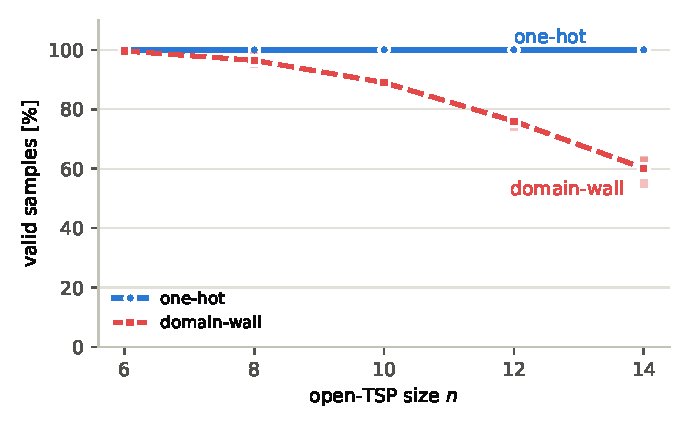
\includegraphics[width=\textwidth]{fig_ablation.pdf}
\caption{Valid-sample fraction under classical SA. Faint points: individual
trials; solid lines: means over 3 trials. Domain-wall saves $n$ variables per
tour but its valid rate decays with $n$ under SA; best-tour quality stayed
comparable (no systematic winner across the 15 runs).}
\label{fig:ablation}
\end{minipage}\hfill
\begin{minipage}[t]{0.49\textwidth}\centering
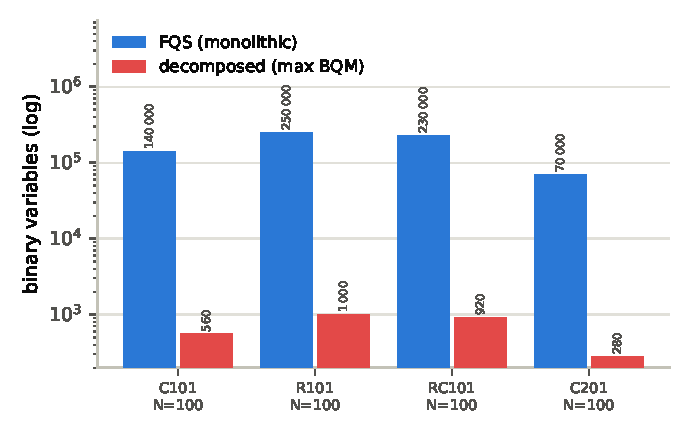
\includegraphics[width=\textwidth]{fig_vars.pdf}
\caption{Largest single sampled BQM, monolithic vs.\ decomposed (log scale).
$N=100$ FQS bars are the computed $MN^2$ equivalent --- unbuildable in
practice, which is exactly the paper's reported limitation.}
\label{fig:vars}
\end{minipage}
\end{figure}

Under classical SA one-hot never produces an invalid sample while domain-wall
degrades from $\sim$99.7\% ($n$=6) to $\sim$60\% ($n$=14) valid. This does
\emph{not} contradict the literature's pro-domain-wall results
(Chen--Stollenwerk--Chancellor 2021): that advantage is a
\emph{hardware-embedding} effect --- the 1-D wall constraints embed with much
shorter chains than one-hot's cliques --- and SA has no embedding. It does
mean the encoding choice must be re-measured on the QPU (valid rate +
chain-break fraction) before trusting either; that is the first thing
\texttt{run\_qpu.py --exp ablation --backend qpu} measures.

\section{Takeaways and next steps}

What survives scrutiny: (i) TW structure can be pushed into both QUBO stages
with zero extra qubits, and the decomposed pipeline stays TW-feasible at
$N=10$ where FQS collapses, reaching a 0.2\% gap to the exact optimum where
one is known (R101-$N$5); (ii) the exact
coarsening rule's no-repair guarantee held on every full-size run; (iii) the
decomposition cuts the largest BQM by 1--3 orders of magnitude. What does not
(yet): domain-wall's variable saving costs valid-sample rate under SA, and at
Solomon-100 scale the classical warm start usually wins. Next, in priority
order: QPU runs of the ablation (settles the encoding question with chain-break
data), QPU runs of Experiment A at $N=10$ (where FQS barely embeds and the
decomposed BQMs embed trivially), a penalty-weight sensitivity sweep (all
weights here are scaled heuristics), and a Benders-style loop feeding realized
route costs back into the assignment QUBO to close the Exp-B gap to the warm
start.

\end{document}
